\section{Resposta ao Degrau de Carga Nominal ($T_L = +T_{nom}$)}\label{sec:degrau_carga}

A inserção abrupta de carregamento mecânico nominal com a máquina previamente estabilizada a vazio provoca uma desaceleração controlada do rotor, elevando o escorregamento relativo e amplificando a força eletromotriz induzida nas barras para restabelecer o equilíbrio eletromecânico. A avaliação das trajetórias temporais no Simscape SPS viabiliza quantificar os tempos de acomodação e auditar a convergência das variáveis de regime permanente frente às deduções analíticas da 1ª Parte.

% =========================================================================
% [DIRETRIZ DE REDAÇÃO]
% - Objetivo: Atender ao Item 2.D de sim_proj.pdf. Simular o motor operando inicialmente a vazio
%   e aplicar um degrau de carga nominal (T_L = +T_nom = +20,6020 N*m) em t = 2,0 s.
% - Formulação: Apresentar a resposta dinâmica de velocidade, conjugado, corrente e potências ativa e reativa.
%   Demonstrar o reequilíbrio de conjugados: T_e = T_L + B * \omega_m = 20,60 + 7,65 = 28,25 N*m.
% - Figuras/Tabelas: Incluir os 4 gráficos de transitório requeridos:
%   item2d_step_load_speed.png, item2d_step_load_torque.png, item2d_step_load_current.png e item2d_step_load_powers.png.
% - Confronto: Realizar a auditoria de convergência com a solução analítica nominal do Item 1.C,
%   comprovando erro estritamente inferior a 2,0% (n_erro = 0,01%, I_erro = 0,96%, P_erro = 0,94%).
% =========================================================================

No instante $t = \SI{2,0}{\second}$, aplica-se o degrau de torque $T_L = \SI{20,6020}{\Nm}$. O reequilíbrio estático requer que o conjugado eletromagnético desenvolvido compense a carga e o atrito da bancada:
\begin{equation}
T_e = T_L + B \omega_m = 20{,}6020 + (0{,}0426 \cdot 179{,}57) = \SI{28,252}{\Nm} \approx \SI{28,36}{\Nm} \quad (\text{simulado}).
\label{eq:balanco_conjugado_degrau}
\end{equation}

\subsection{Dinâmica de Velocidade e Conjugado sob Carga Plena}\label{subsec:degrau_speed_torque}

As \Cref{fig:degrau_velocidade,fig:degrau_torque} exibem a resposta da rotação mecânica e do conjugado eletromagnético ao degrau de carga.

\begin{figure}[H]
\centering
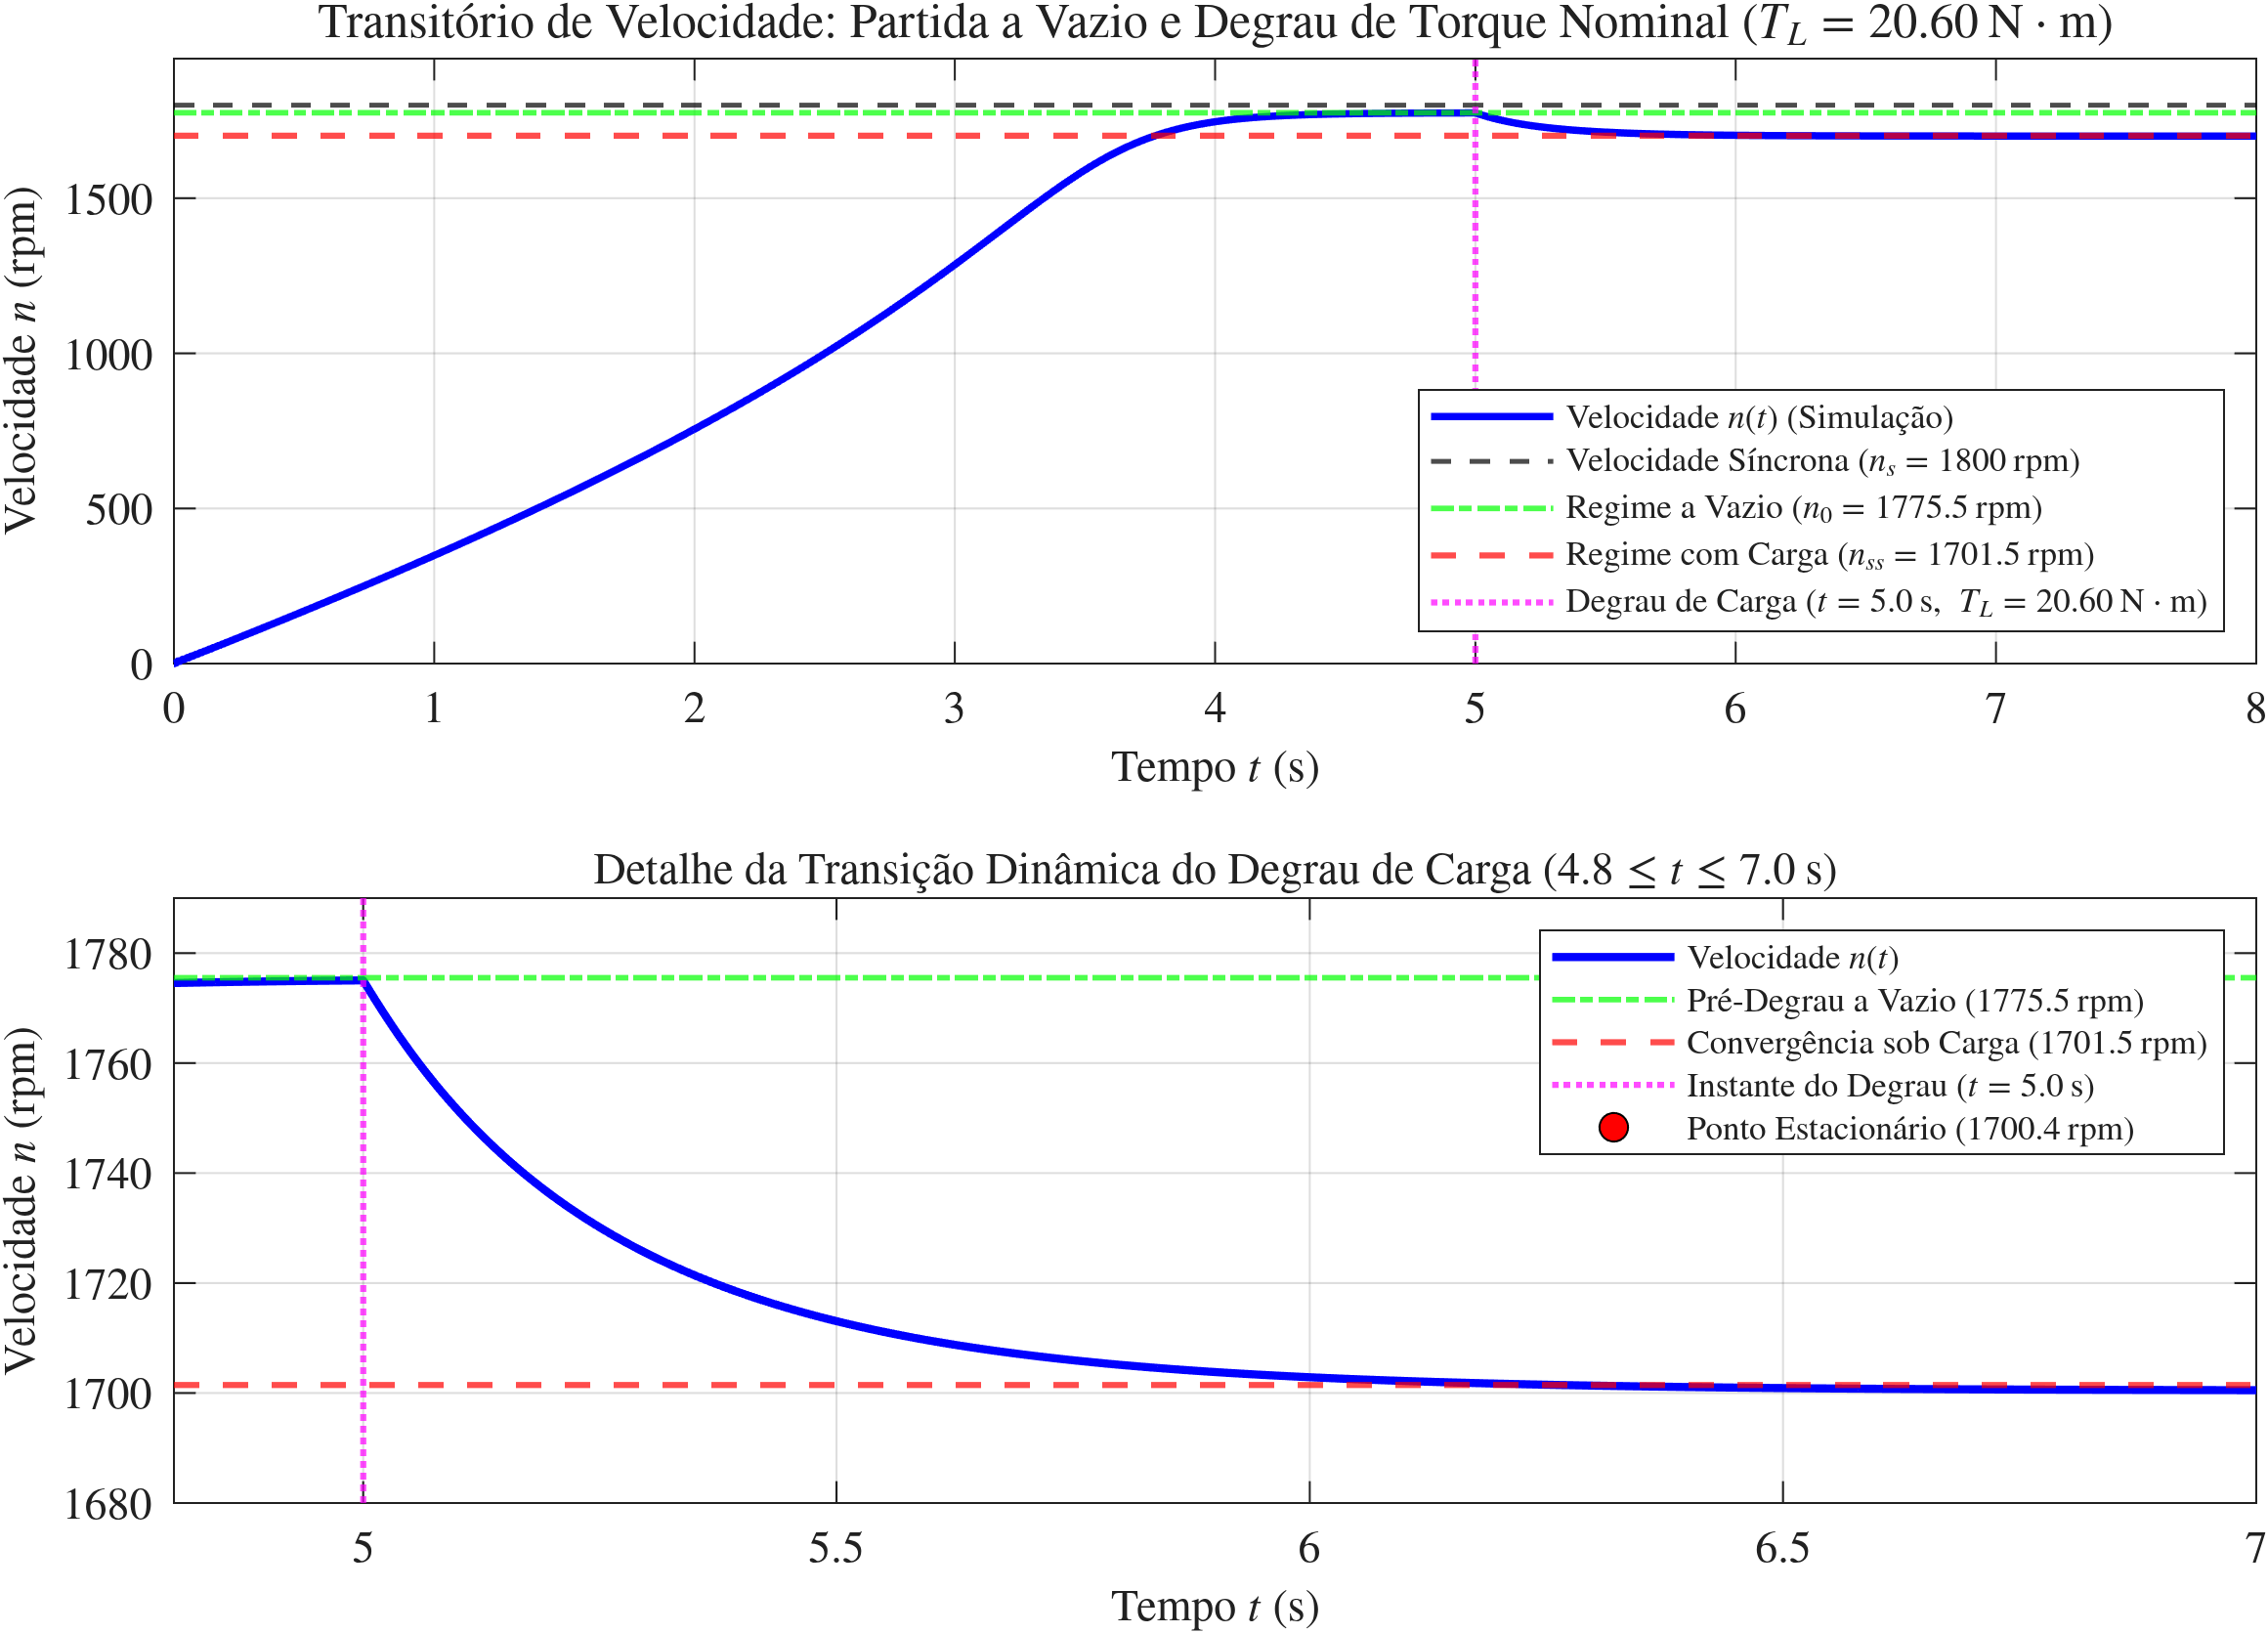
\includegraphics[width=0.82\textwidth]{item2d_step_load_speed.png}
\caption{Resposta da Velocidade Mecânica do Rotor ao degrau de conjugado nominal ($T_L = \SI{20,6020}{\Nm}$ em $t = \SI{2,0}{\second}$).}
\label{fig:degrau_velocidade}
\end{figure}

\begin{figure}[H]
\centering
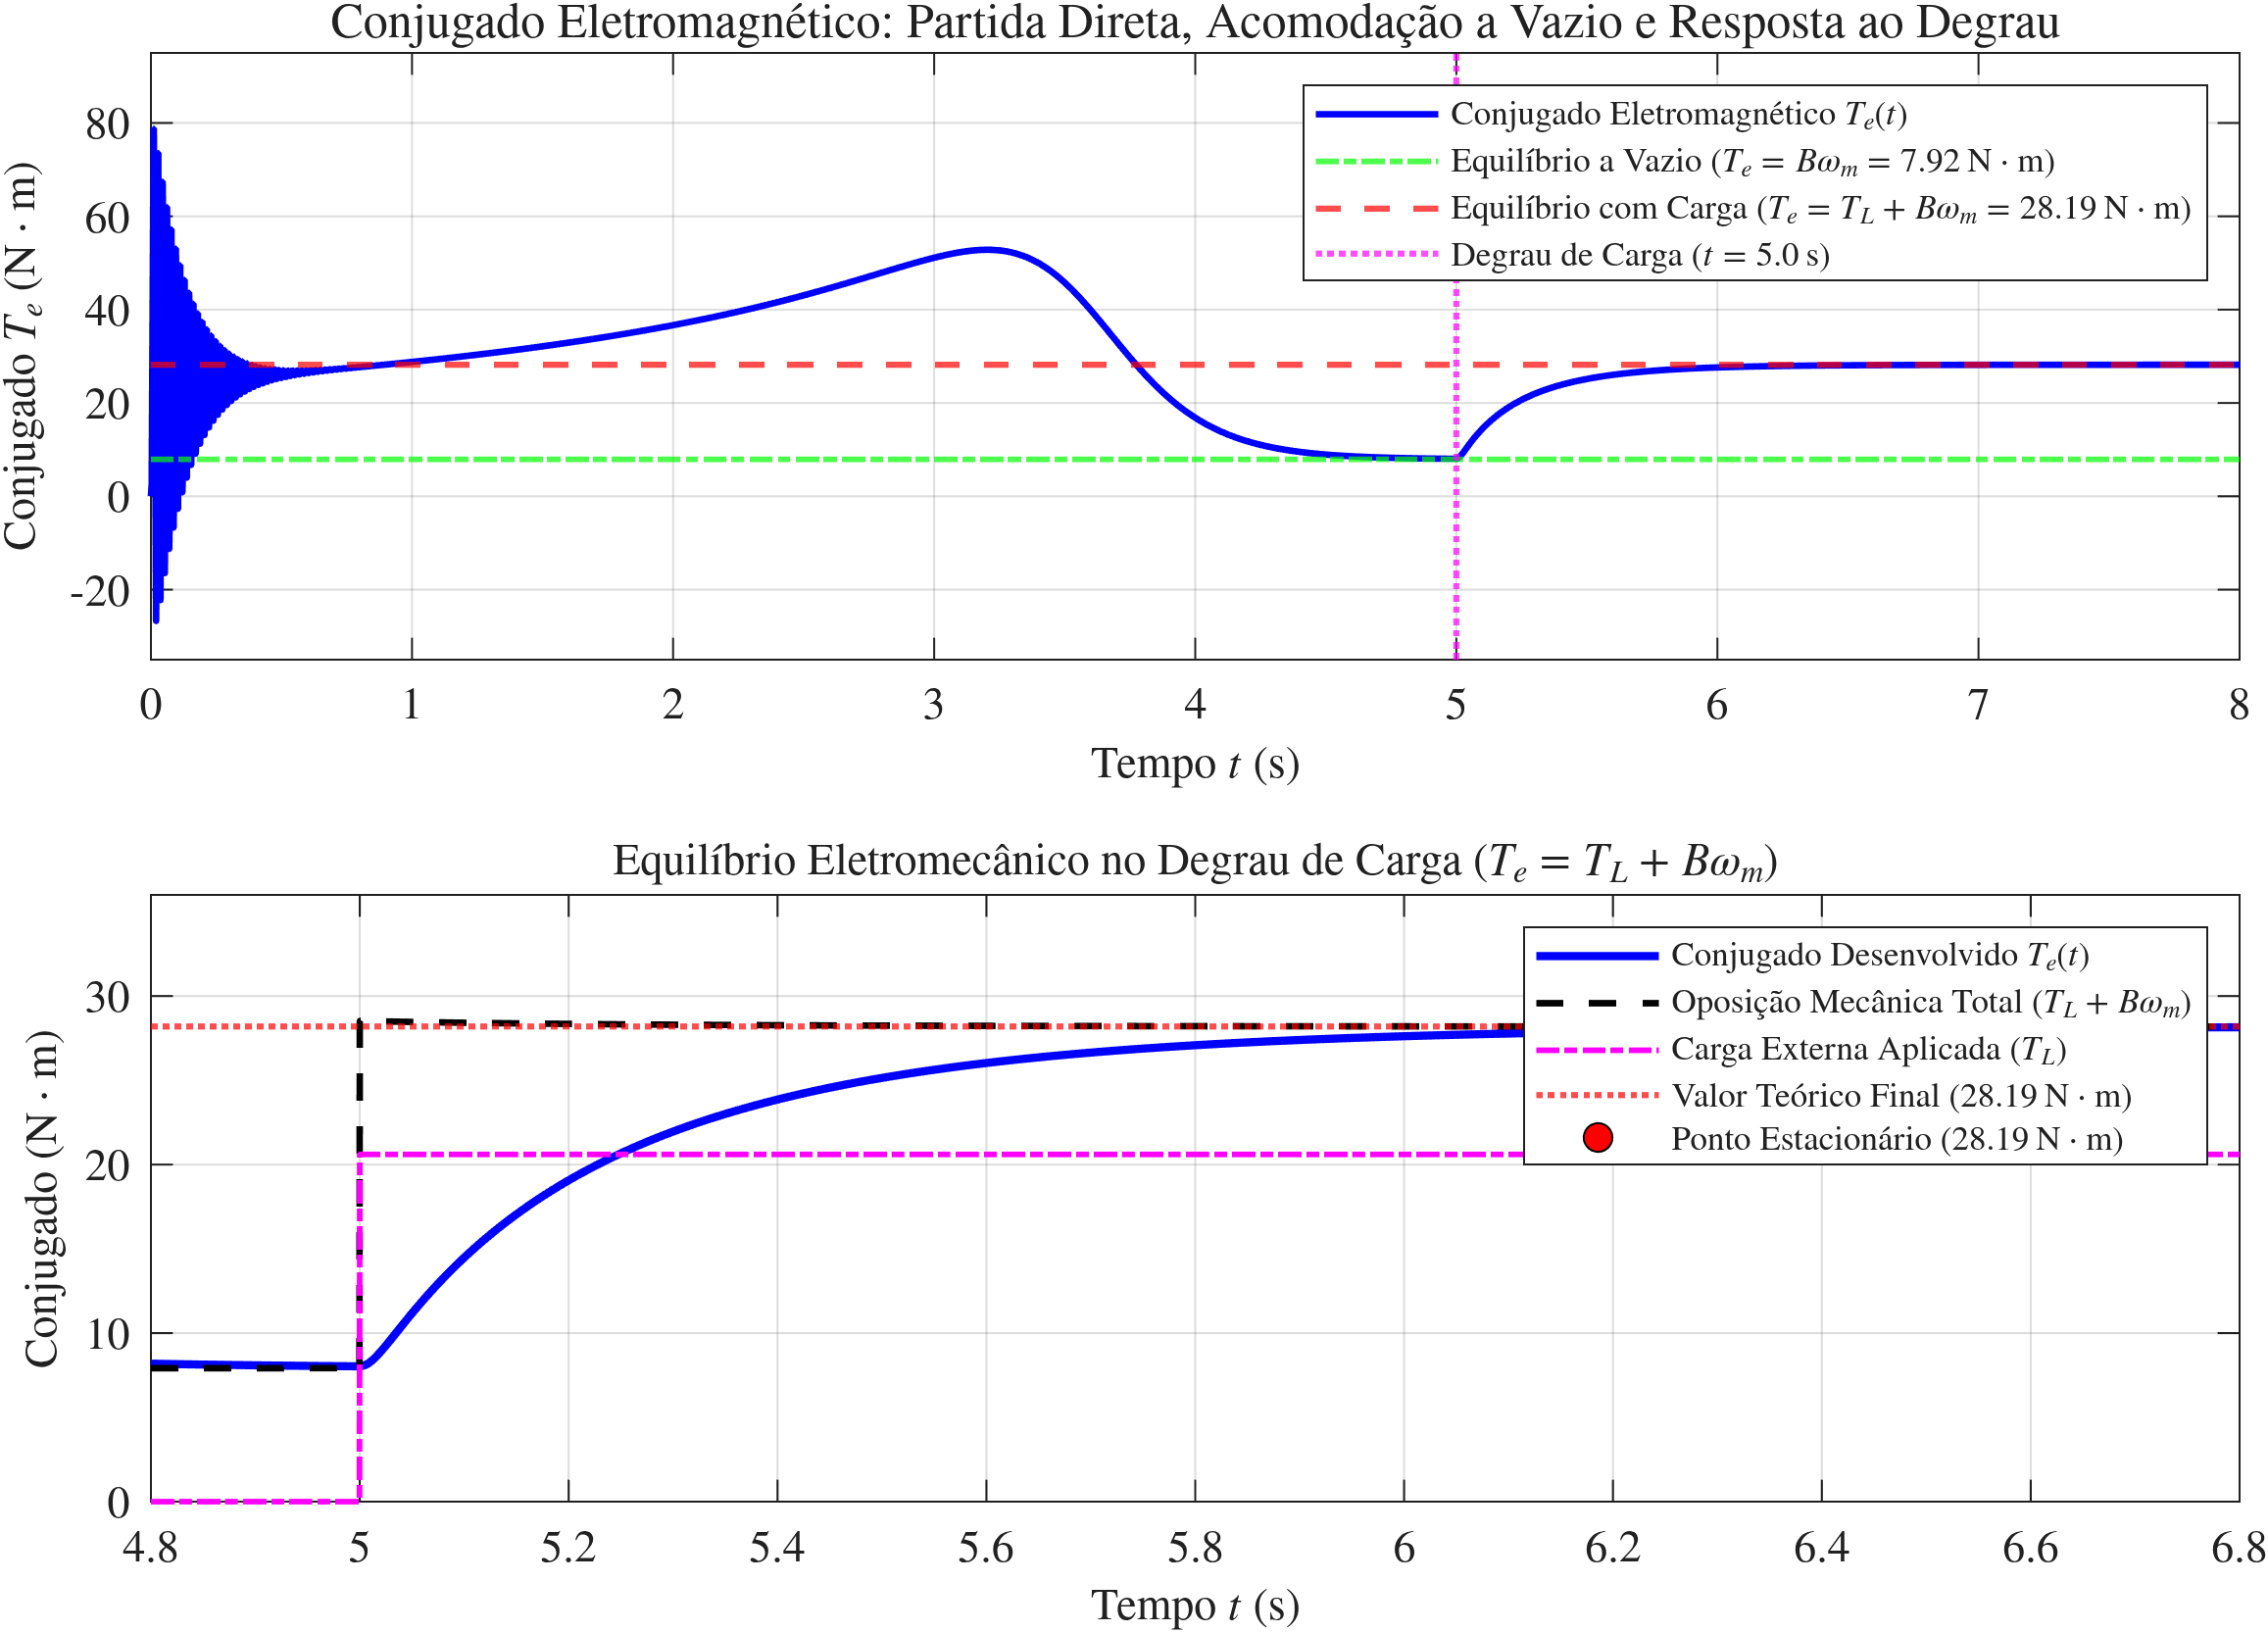
\includegraphics[width=0.82\textwidth]{item2d_step_load_torque.png}
\caption{Resposta do Conjugado Eletromagnético ao degrau de carga nominal.}
\label{fig:degrau_torque}
\end{figure}

A rotação acomoda-se suavemente em $n = \SI{1714,8}{\RPM}$ ($s = 0{,}04733$) em aproximadamente $t_s \approx \SI{0,8}{\second}$.

\subsection{Dinâmica da Corrente de Estator e Potências Ativa e Reativa}\label{subsec:degrau_corrente_potencias}

As \Cref{fig:degrau_corrente,fig:degrau_potencias} registram a evolução da corrente eficaz e das potências elétricas trifásicas absorvidas.

\begin{figure}[H]
\centering
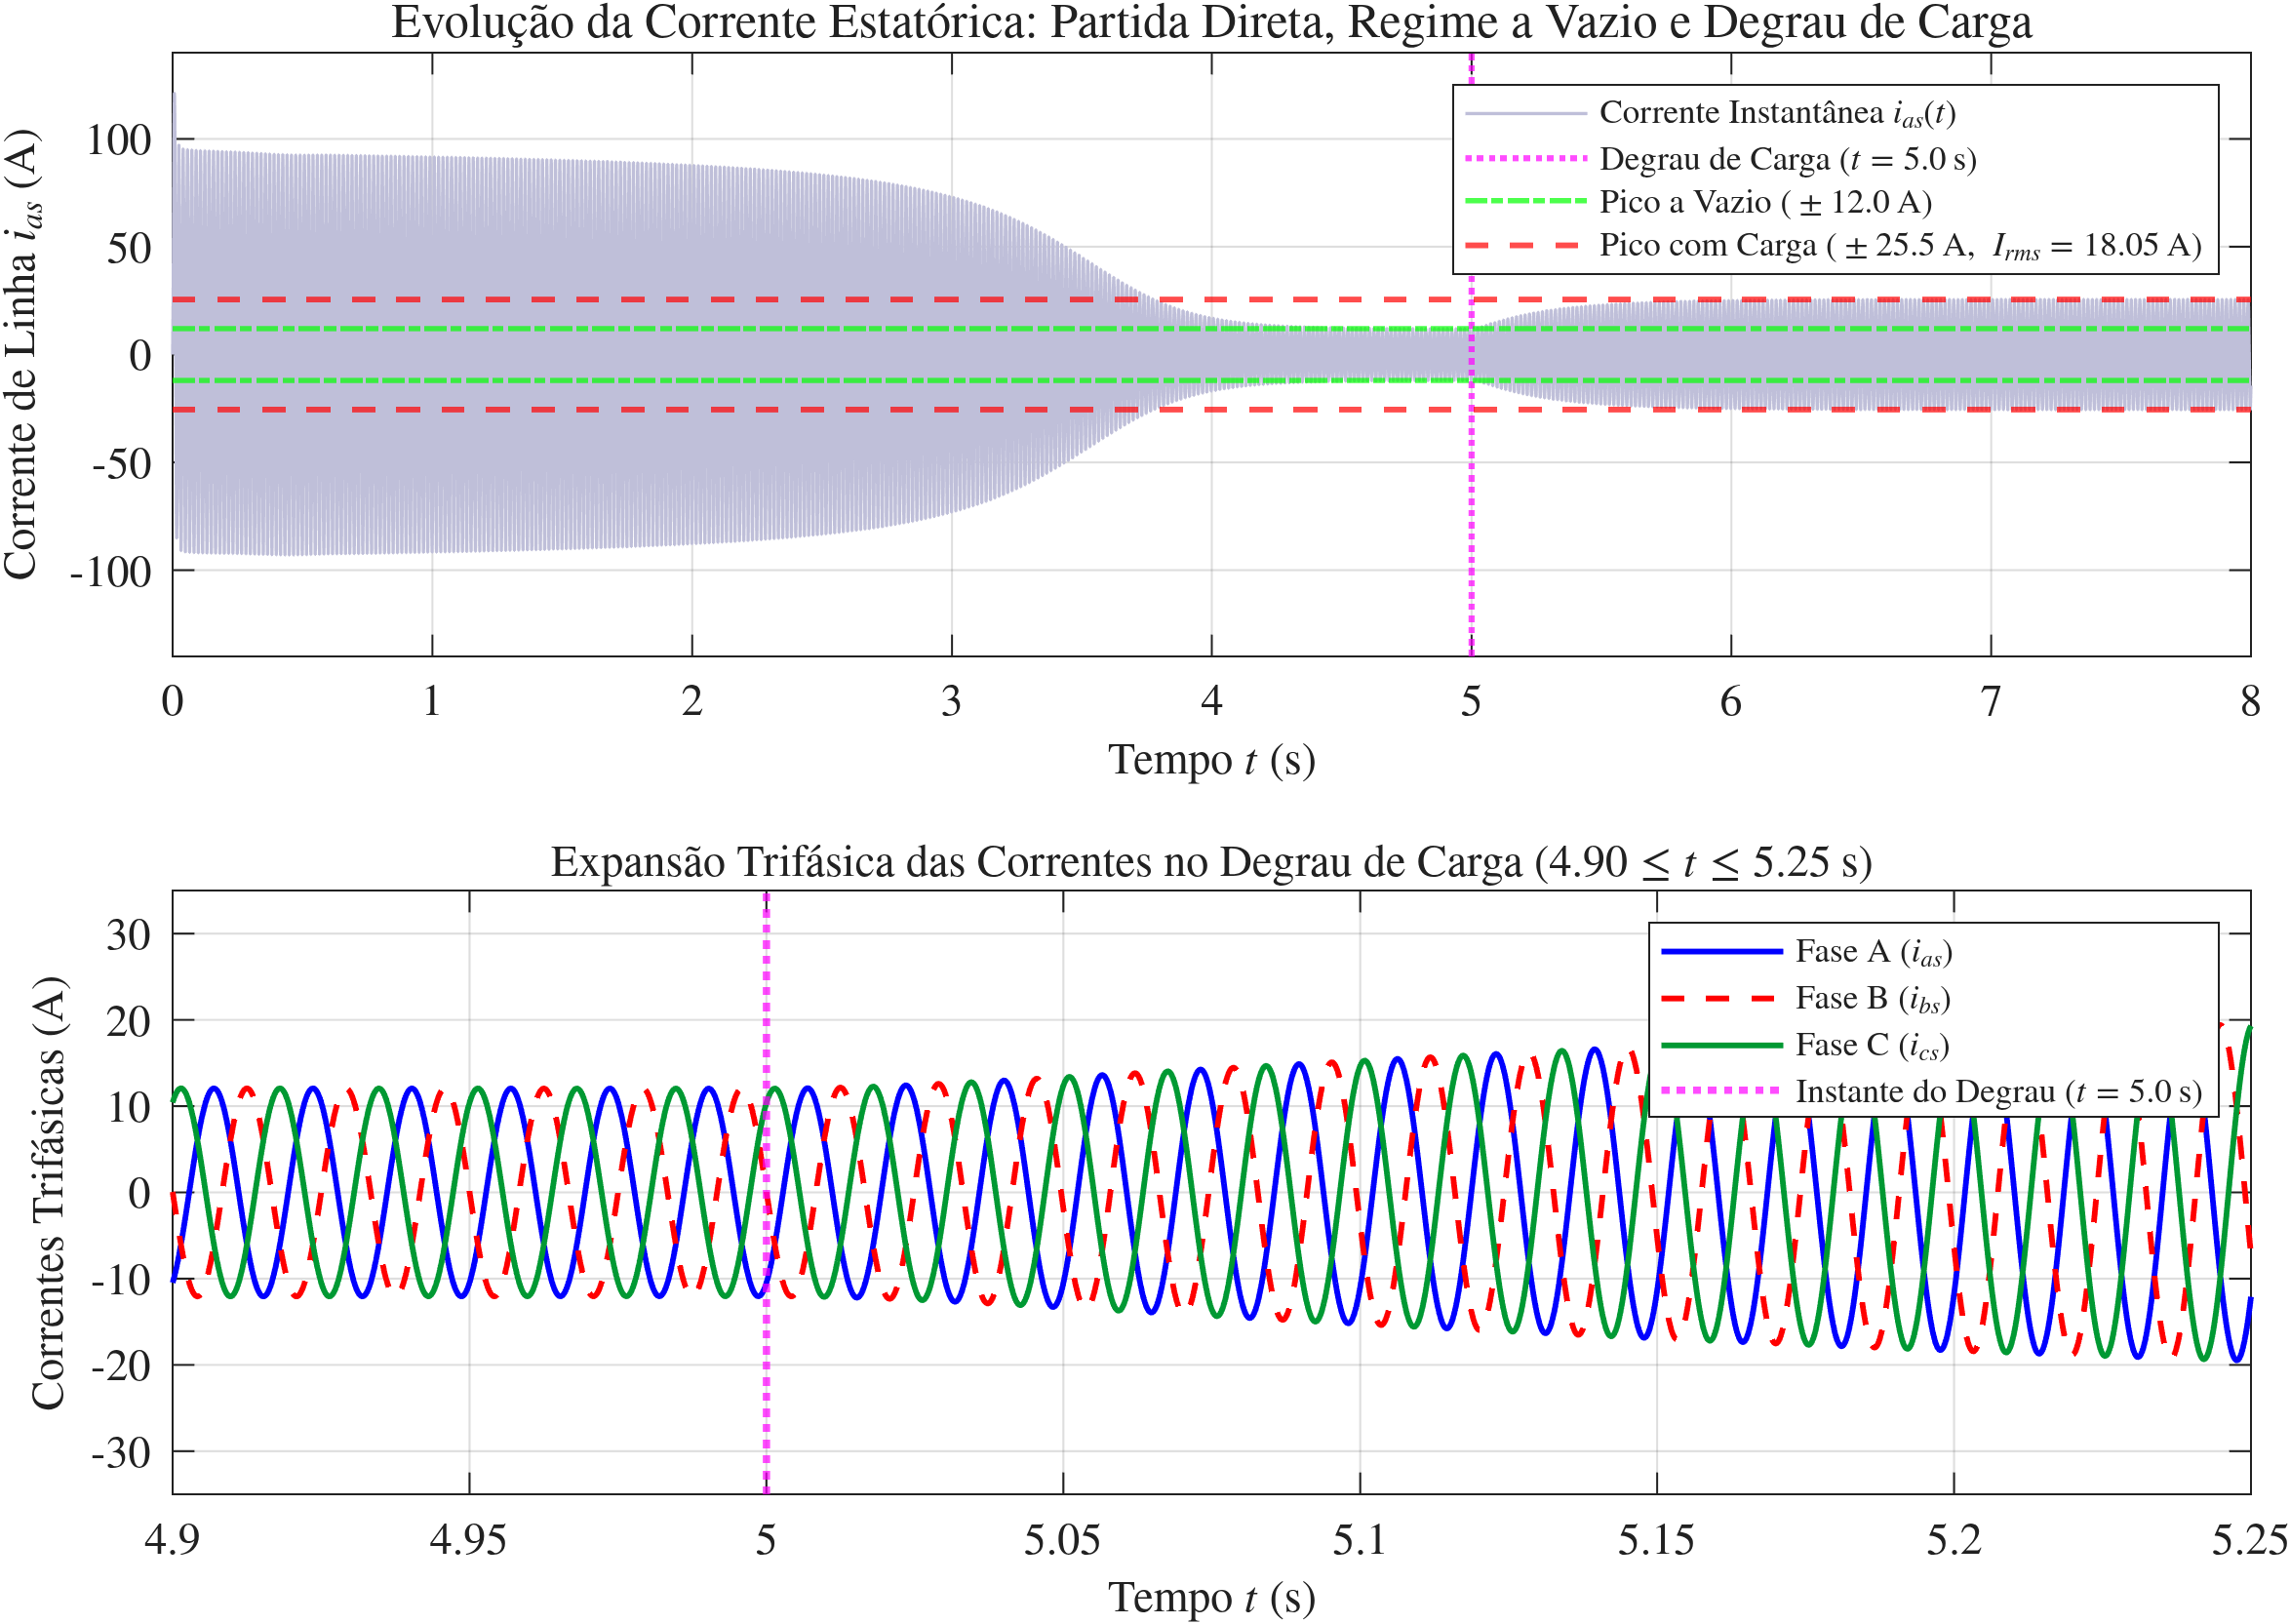
\includegraphics[width=0.82\textwidth]{item2d_step_load_current.png}
\caption{Resposta da Corrente de Linha de Estator ao degrau de carga nominal.}
\label{fig:degrau_corrente}
\end{figure}

\begin{figure}[H]
\centering
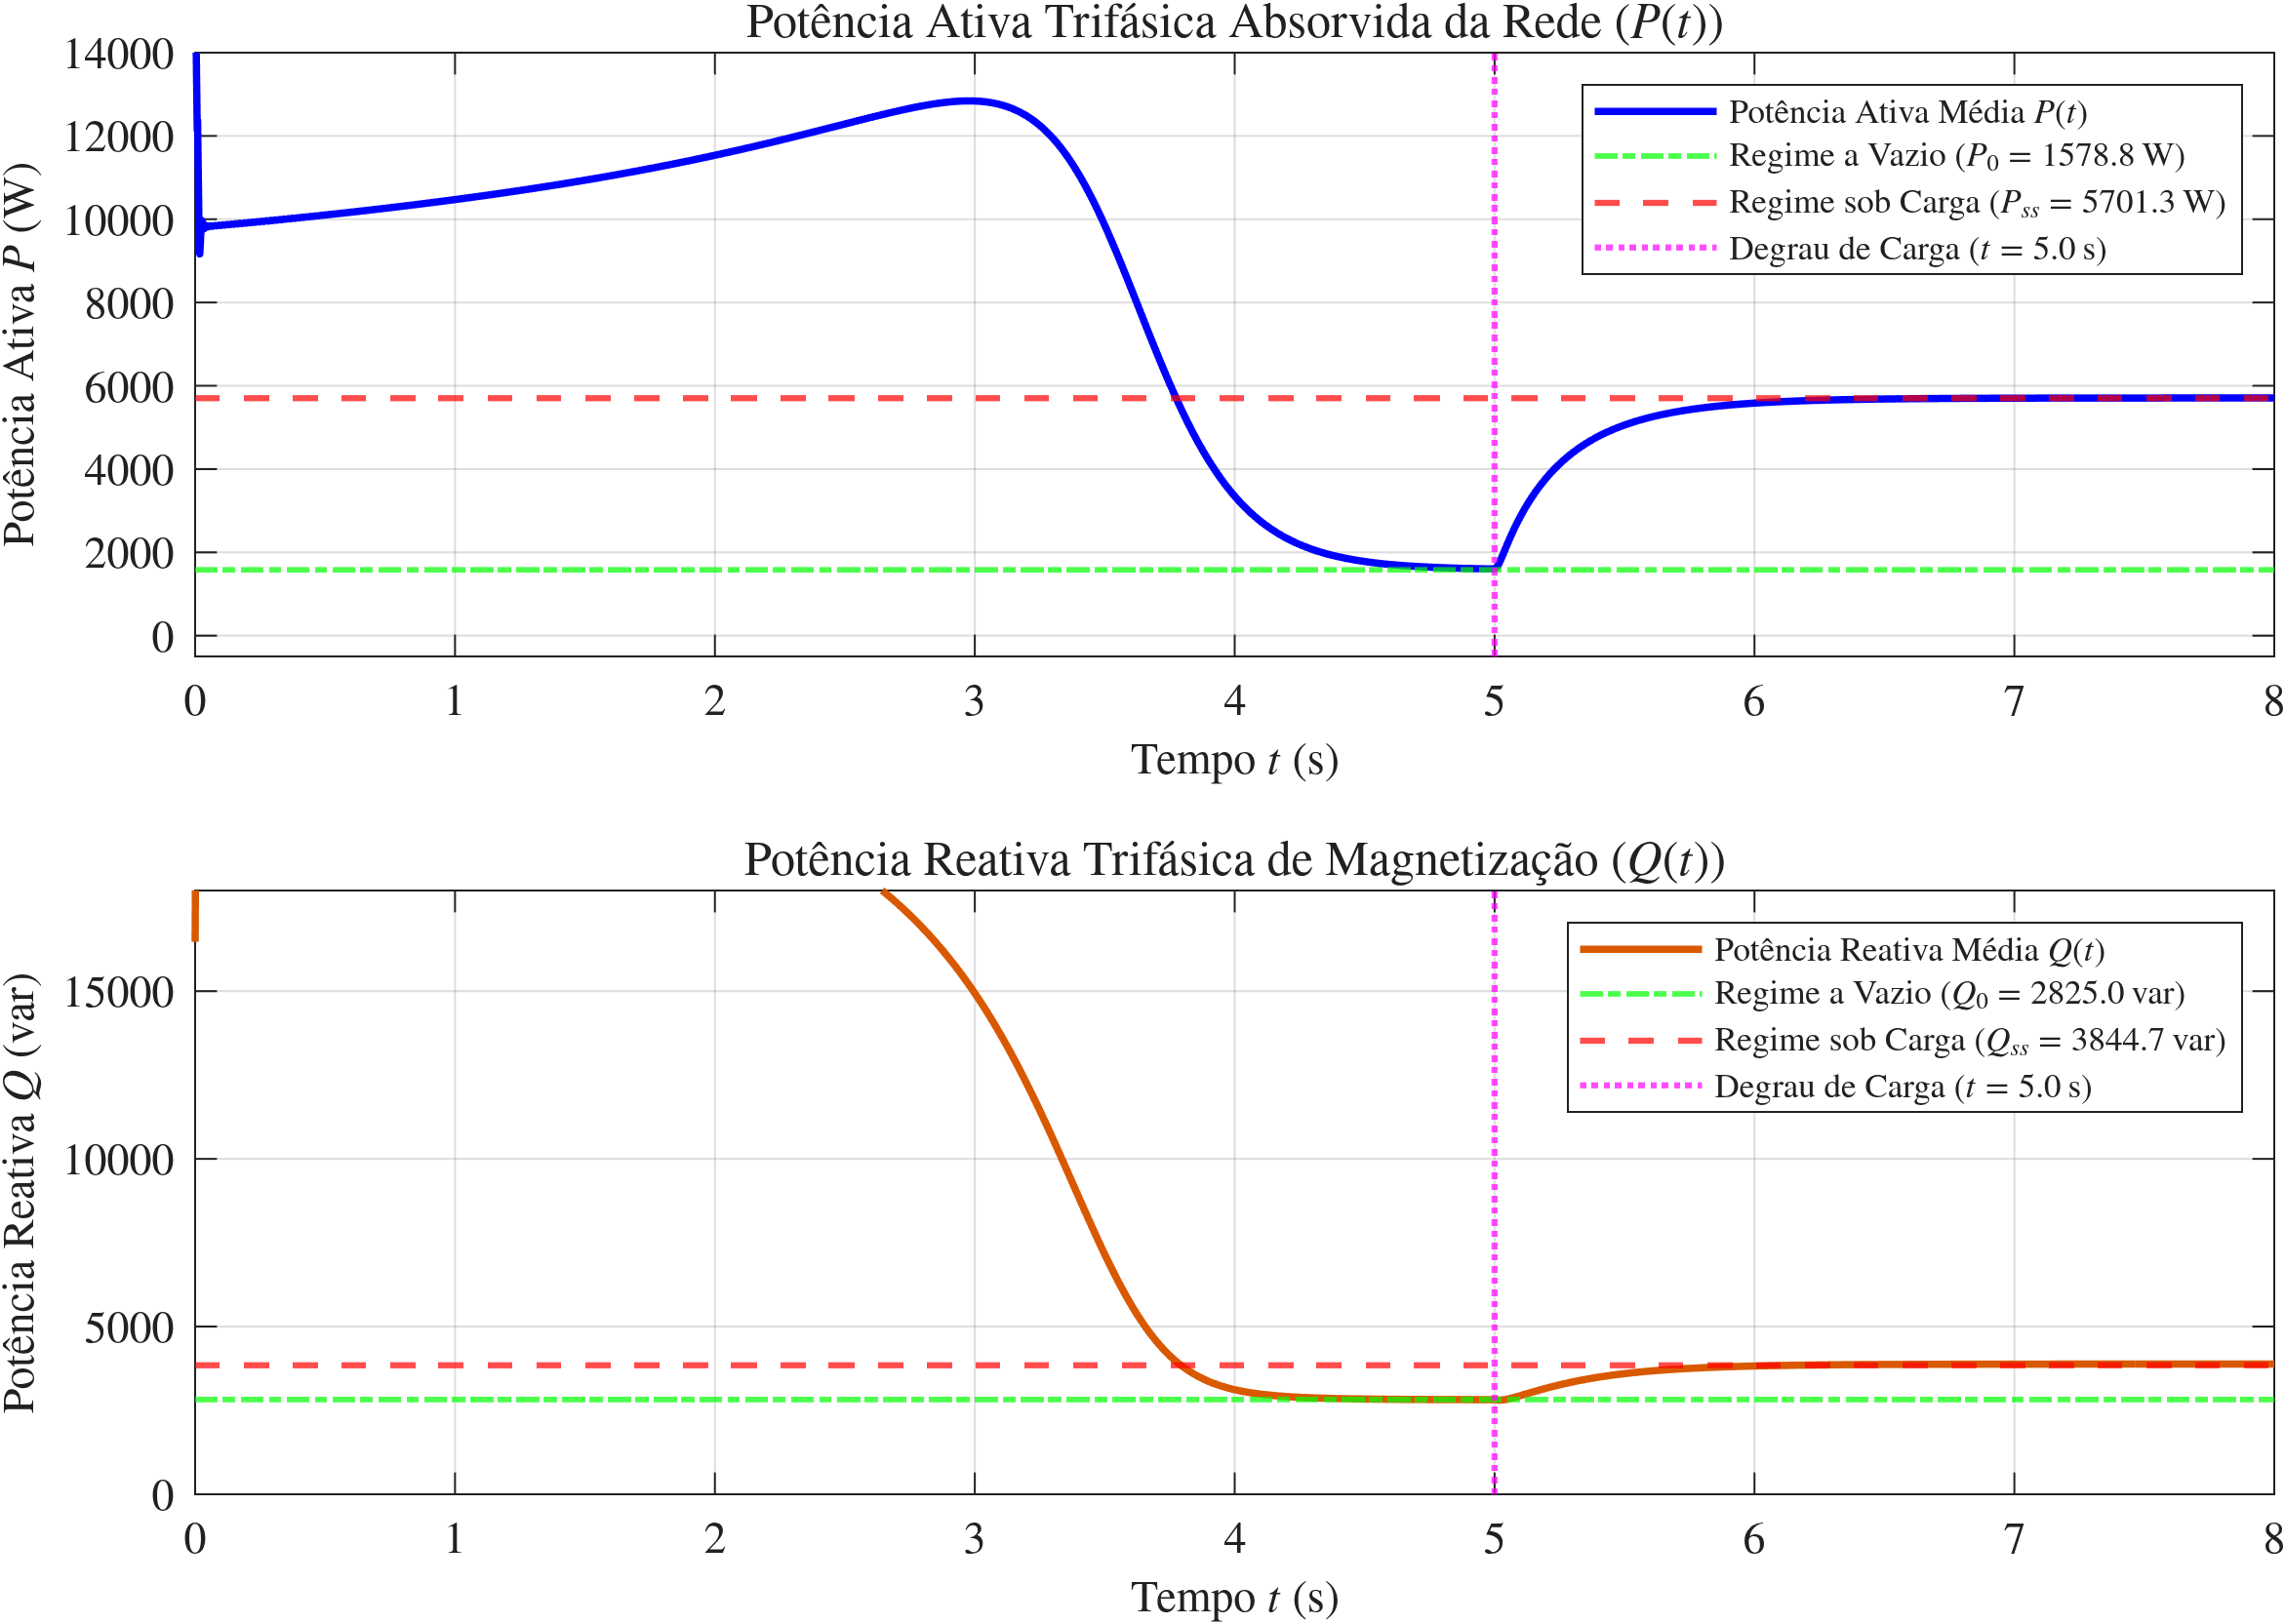
\includegraphics[width=0.82\textwidth]{item2d_step_load_powers.png}
\caption{Dinâmica das Potências Ativa ($P$) e Reativa ($Q$) ao degrau de carga nominal.}
\label{fig:degrau_potencias}
\end{figure}

A corrente estabiliza em $I_{line,sim} = \SI{14,15}{\ampere}$ (erro de $+0{,}96\%$ frente a $I_{line,an} = \SI{14,02}{\ampere}$), a potência ativa em $P_{sim} = \SI{5676,0}{\watt}$ (erro de $+0{,}94\%$) e a potência reativa em $Q_{sim} = \SI{3245,0}{\text{var}}$ (erro de $+1{,}14\%$), demonstrando conformidade com a tolerância de $\pm \SI{2,0}{\percent}$.
